% Fase 3B, exemplos 5–6. Fontes: mb-uso/secoes.
\begin{frame}[fragile]{Exemplo 5 — Incorporar um problema criado pelo pesquisador}
\begin{columns}[T,onlytextwidth]
\begin{column}{.52\textwidth}
\textbf{Problema próprio:} 3 objetivos, 10 variáveis de decisão. A avaliação vetorizada transforma matrizes de decisão em matrizes de objetivos.
\begin{lstlisting}[style=python,basicstyle=\ttfamily\fontsize{6.9}{8.3}\selectfont]
class MyProblem(mb.mops.BaseMop):
    def evaluation(self, X,
                   n_ieq_constr=0):
        theta = X[:, :2] * (np.pi/2)
        g = np.sum(
            (X[:, 2:] - 0.5)**2, axis=1)
        f1 = (1+g)*np.cos(theta[:,0]) \
             *np.cos(theta[:,1])
        f2 = (1+g)*np.cos(theta[:,0]) \
             *np.sin(theta[:,1])
        f3 = (1+g)*np.sin(theta[:,0])
        return {'F': np.column_stack(
            [f1, f2, f3])}
\end{lstlisting}

\end{column}
\begin{column}{.46\textwidth}
\textbf{Intuição geométrica:} as oito últimas variáveis determinam o afastamento radial
\[
 g=\sum_{j=3}^{10}(x_j-0{,}5)^2.
\]
Quando $x_j=0{,}5$ para $j\geq 3$, $g=0$ e a frente adquire a geometria do octante esférico.
\par\smallskip
A classe completa também implementa \texttt{\_\_init\_\_()} e \texttt{ps()}. A mesma infraestrutura analisa o MOP definido pelo usuário.
\end{column}
\end{columns}
\end{frame}

\begin{frame}[fragile]{Exemplo 5 — O MOP personalizado usa a mesma API}
\begin{columns}[T,onlytextwidth]
\begin{column}{.36\textwidth}
\begin{lstlisting}[style=python,basicstyle=\ttfamily\fontsize{8}{10}\selectfont]
mop = MyProblem()
mop.calibrate()
exp.mop = mop
exp.run()
mb.view.topology(exp)
\end{lstlisting}
\textbf{Resultado:} 200 soluções não dominadas na população final.
\par\smallskip
A distribuição acompanha a superfície esférica de referência. A busca encontra soluções próximas da condição $g=0$, mesmo sendo um problema definido fora do catálogo.
\end{column}
\begin{column}{.62\textwidth}
\centering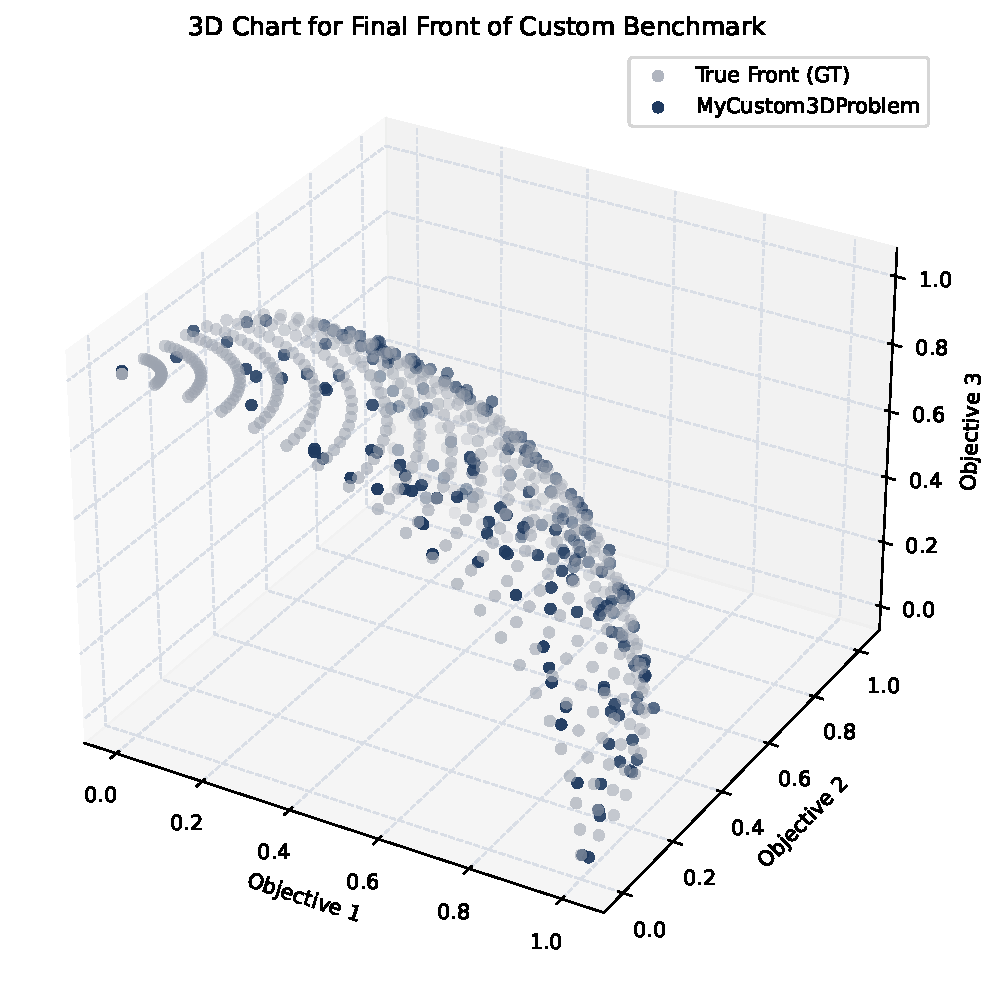
\includegraphics[width=\linewidth,height=.64\textheight,keepaspectratio]{figures/example_05_01_topology.pdf}

\end{column}
\end{columns}
\vspace{.06cm}\textbf{Significado:} avaliação, calibração, execução e análise são reaproveitadas sem redefinir todo o ambiente experimental.
\end{frame}

\begin{frame}[fragile]{Exemplo 6 — Uma diferença nas médias é consistente?}
\textbf{Protocolo:} DTLZ2; dez execuções de NSGA-III e dez de SPEA2; análise do HV final sob referência compartilhada.
\begin{columns}[T,onlytextwidth]
\begin{column}{.57\textwidth}
\begin{lstlisting}[style=python,basicstyle=\ttfamily\fontsize{7.6}{9.5}\selectfont]
shift = mb.stats.perf_shift(
    exp1, exp2, metric=mb.metrics.hv)
match = mb.stats.perf_match(
    exp1, exp2, metric=mb.metrics.hv)
win = mb.stats.perf_win(
    exp1, exp2, metric=mb.metrics.hv)
shift.report()
match.report()
win.report()
\end{lstlisting}
\end{column}
\begin{column}{.41\textwidth}
\textbf{HV médio final}
\par\smallskip NSGA-III: \textbf{0,910163}
\par SPEA2: \textbf{0,908959}
\par\medskip
A diferença observada é de aproximadamente \textbf{0,0012}. Uma comparação das médias, sozinha, não informa se a separação é sistemática.
\end{column}
\end{columns}
\vspace{.1cm}\textbf{Pergunta central:} os valores de uma distribuição tendem realmente a superar os da outra, ou as execuções se sobrepõem?
\end{frame}

\begin{frame}{Exemplo 6 — Três perspectivas estatísticas da mesma comparação}
\renewcommand{\arraystretch}{1.4}
\begin{tabularx}{\linewidth}{@{}>{\bfseries}p{.25\linewidth}p{.17\linewidth}X@{}}
Mann--Whitney & $p=0{,}570750$ & Compara posições relativas dos HVs ordenados. Não há evidência de deslocamento consistente neste ensaio.\\
KS & $p=0{,}786930$ & Compara as distribuições acumuladas. Não se observa separação convincente de forma ou posição.\\
$A_{12}$ & $0{,}58$ & Em pares de execuções sorteadas, NSGA-III supera SPEA2 com frequência estimada de 58\% (com empates divididos).\\
\end{tabularx}
\vspace{.13cm}
\textbf{Interpretação:} os algoritmos apresentaram desempenho final semelhante nessas dez execuções, apesar da pequena vantagem ordinal do NSGA-III.
\par{\scriptsize Valores de $p$ elevados não demonstram igualdade dos algoritmos.}
\end{frame}
